\documentclass[12pt, a4paper]{article}
\usepackage[utf8]{inputenc}

% Format
\usepackage{layout}
\setlength{\parindent}{0.5in}
\setcounter{secnumdepth}{0}
\usepackage{lineno}

% Font
\usepackage{MinionPro}
\input glyphtounicode
\pdfgentounicode=1
\usepackage{microtype}
\usepackage[super]{nth}
\usepackage{tfrupee}

% Language
\usepackage[british]{babel}

% References
\usepackage[nosectionbib, tocbib, unnumberedbib]{apacite}

% Figures
\usepackage{graphicx}
\usepackage[small, labelfont=it, labelsep=period]{caption}

% Tables
\usepackage{booktabs}
\usepackage{tabularx}

% Commands
\newcommand{\pest}[4]{$ \text{Pr} (\text{``us''} | \text{#1}) = #2$, $[#3, #4]$}
\newcommand{\pdif}[4]{$ \Delta\text{Pr} (\text{``us''} | \text{#1}) = #2$, $[#3, #4]$}

% Frontmatter
\title{Intergroup contact fosters\\more inclusive social identities}
\date{August 23, 2018}

\begin{document}

\begin{figure}
\centering
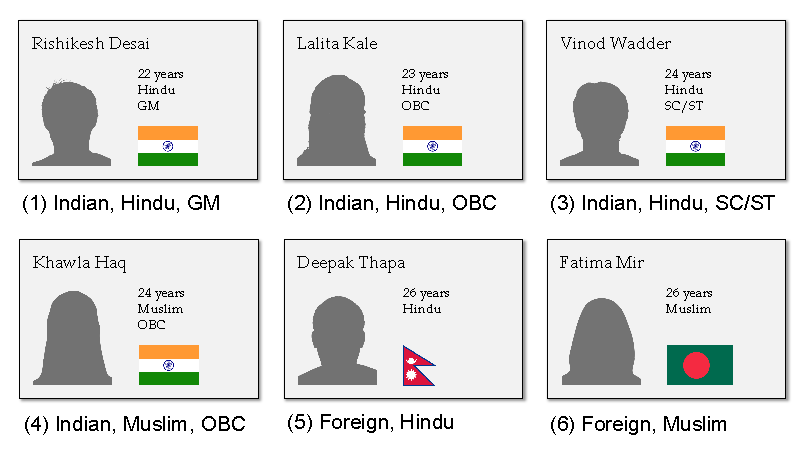
\includegraphics[scale=1]{../figures/figure-1}
\caption{
Schematic representations of social identity structures, ordered by social identity inclusiveness. Shaded regions represent the groups which a participant has to categorize as ``us'' to be assigned that structure. An Indian Hindu, for example, may consider only people who share their nationality, religion, and caste as ingroup members (intersection). Someone else may consider all their fellow Indians, whatever their religion or caste, as ingroup members (dominance). Another person may consider anyone who shares their nationality or religion as ingroup members (merger).
}
\label{fig:f1}
\end{figure}

\begin{table}    
\caption[Participants by gender, age, nationality, religion, and caste]{Participants by gender, age, nationality, religion, and caste. Categories in \textit{italics} were excluded from the final sample. N/A marks missing responses.}
\centering
\figureversion{lining, tabular}
\small	
\begin{tabular}{llrr} \addlinespace \toprule
\multicolumn{2}{l}{Category} & $n$ & \% \\ \midrule \addlinespace 
Gender      & Woman      & 215 & 61 \\
            & Man & 121 & 34 \\
            & Other & 0 & 0 \\
            & N/A & 15 & 4 \\ \addlinespace \addlinespace
Age         & 18--20 & 1 & 0 \\
            & 21--23 & 254 & 72 \\
            & 24--26 &  77 & 22 \\
            & 27--29 &  10 &  3 \\
            & 30--32 &   1 &  0 \\
            & 33--35 &   0 &  0 \\
            & 36 or older & 1 & 0 \\ 
            & N/A & 7 & 2 \\ \addlinespace \addlinespace
Nationality & Indian & 339 & 97 \\
            & Other & 0 & 0 \\
            & N/A & 12 & 3 \\ \addlinespace \addlinespace
Religion    & Buddhism & 1 & 0 \\ 
            & Christianity & 11 & 3 \\ 
            & Hinduism & 297 & 85 \\ 
            & \textit{Islam} & \textit{27} & \textit{8} \\ 
            & Jainism & 8 & 2 \\ 
            & Other & 2 & 1 \\ 
            & N/A & 5 & 1 \\ \addlinespace \addlinespace
Caste       & General Caste & 104 & 30 \\ 
            & Other Backward Class & 143 & 41 \\ 
            & Scheduled Caste & 54 & 15 \\ 
            & Scheduled Tribe & 23 & 7 \\ 
            & \textit{Other / Not applicable} & \textit{20} & \textit{6} \\ 
            & \textit{N/A} & \textit{7} & \textit{2} \\ \addlinespace \midrule
Total       &   & 351 & 100 \\ \bottomrule
\end{tabular}
\label{tab:t1}
\end{table}

\begin{figure}
\centering
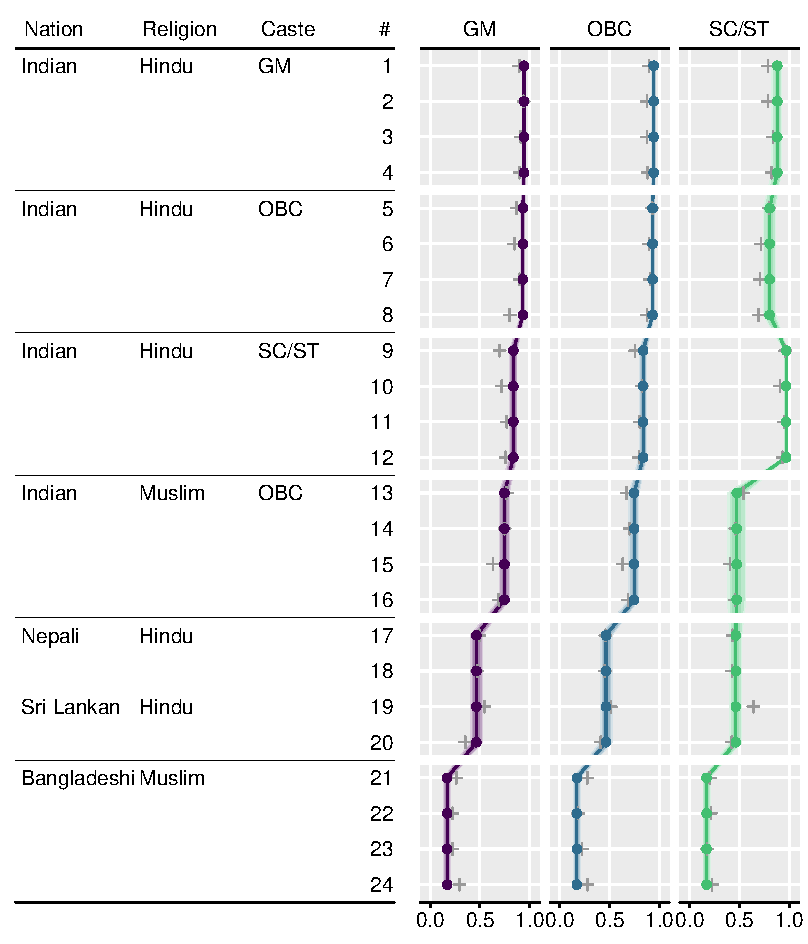
\includegraphics[scale=1]{../figures/figure-2}
\caption{Examples of targets used in the triple crossed-categorization task. Based on ratings in a pilot study ($N = 26$), we selected the four most prototypical targets (out of fifty initial targets) for each of six plausible combinations of caste, religion, and nationality (for details, see Appendix~A). Each target showed a person's caste (GM = General Merit, OBC = Other Backward Class, SC/ST = Scheduled Caste/Scheduled Tribe), religion (Hindu, Muslim), and nationality (Indian, Nepali, Sri Lankan, Bangladeshi). Each target also showed the person's first and last name, age (21--26 years), and a silhouette corresponding to the person's gender (adapted from Ma, Correll \& Wittenbrink, 2015). Each target's age and silhouette, as well as the order in which the targets were presented, varied across sessions.}
\label{fig:f2}
\end{figure}

\begin{table}
\caption{
Comparison of models estimating the probability of participants categorising targets as ``us'' versus ``not us''. $\textit{ELPD}$ is the expected log predictive density, with higher numbers indicating that a model is expected to make more accurate out-of-sample predictions (Vehtari, Gelman, \& Gabry, 2017). $\Delta\textit{ELPD}$ is the difference in $\textit{ELPD}$ between the current and previous model, with positive values indicating that the current model is expected to make more accurate out-of-sample predictions. We selected a more complex model over a simpler model when $\frac{\Delta\textit{ELPD}}{\textit{SE}} \geq 2$. $w$ are stacking weights based on the models' expected log predictive densities (Yao et al., 2018).% Appendix~X describes all models in detail.
}
\centering
\figureversion{lining, tabular}
\small
\begin{tabularx}{\linewidth}{r@{~}rXrrrrrr} \toprule
\# &  & Description & $\textit{ELPD}$ & $\textit{SE}$ & $\Delta\textit{ELPD}$ & $\textit{SE}$ & $\frac{\Delta\textit{ELPD}}{\textit{SE}}$ & $w$ \\ \midrule 
0 &      & Intercept (Participant) & -4703.5 & 23.7 &     - &    - &    - & .00 \\ 
1 & vs 0 & Intercept (Category)    & -3853.5 & 41.6 & 850.1 & 37.4 & 22.7 & .00 \\
2 & vs 1 & Group differences (SC/ST)       & -3791.3 & 42.0 &  62.1 & 11.1 &  5.6 & .00 \\
3 & vs 2 & Group differences (OBC)         & -3792.1 & 42.2 &  -0.8 &  3.6 & -0.2 & .07 \\ \midrule
4 & vs 2 & Intergroup contact (4) & -3743.4 & 42.8 &  47.9 &  8.8 &  5.4 & .00 \\
5 & vs 4 & Intergroup contact (2) & -3736.7 & 42.6 &   6.7 &  1.8 &  3.8 & .92 \\
6 & vs 5 & Intergroup contact (2) & -3747.8 & 42.7 & -11.1 &  3.2 & -3.5 & .00 \\
7 & vs 2 & Social dominance orientation & -3791.0 & 42.1 &   0.4 &  3.3 &  0.1 & .00 \\
\bottomrule
\end{tabularx}
\label{tab:t2}
\end{table}

\begin{figure}
\centering
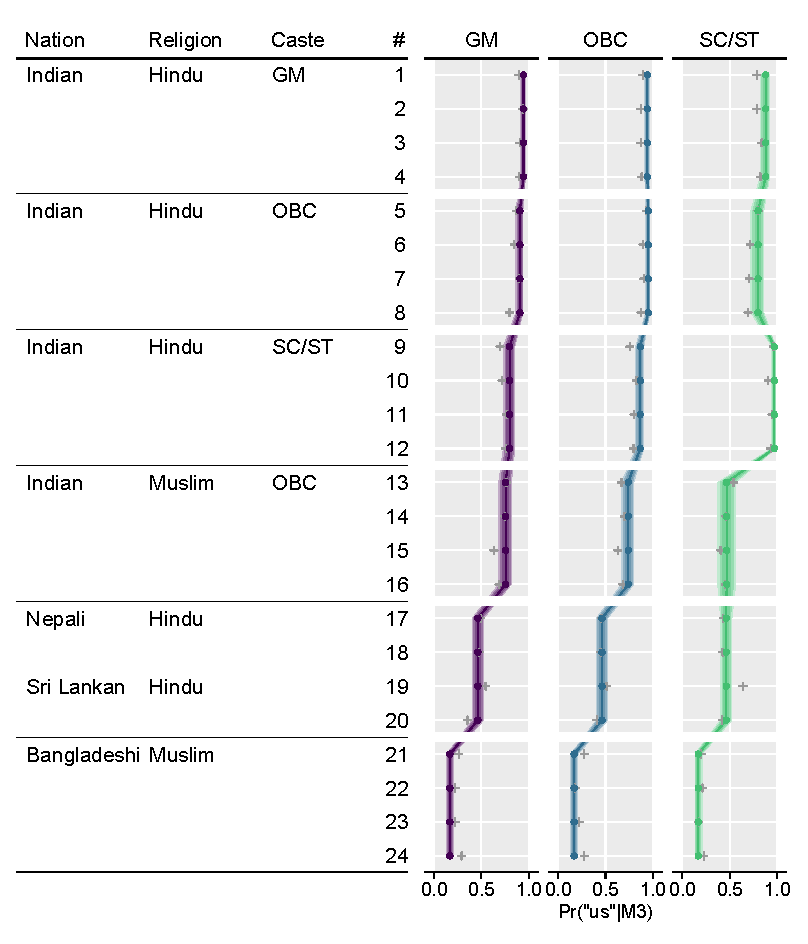
\includegraphics[scale=1]{../figures/figure-3}
\caption{
Estimated probability of participants categorizing a target as ``us'' versus ``not us'' by targets' nationality, religion, and caste (vertical), and participants' caste membership (horizontal). Dots (•) indicate the most plausible \emph{estimate} for a given target's probability of being included in participants' ingroup (in Model~2, Table~\ref{tab:t2}), while the shaded ribbons encompass the 67\% (darkest shade), 89\%, and 97\% (lightest shade) most plausible estimates of that probability. Pluses (+) indicate the \emph{observed} proportion of participants who included a given target in their ingroup. Comparing predicted and observed proportion shows that the model represents the data reasonably well. GM = General Merit, OBC = Other Backward Class, SC/ST = Scheduled Caste/Scheduled Tribe.
}
\label{fig:f3}
\end{figure}

\begin{figure}
\centering
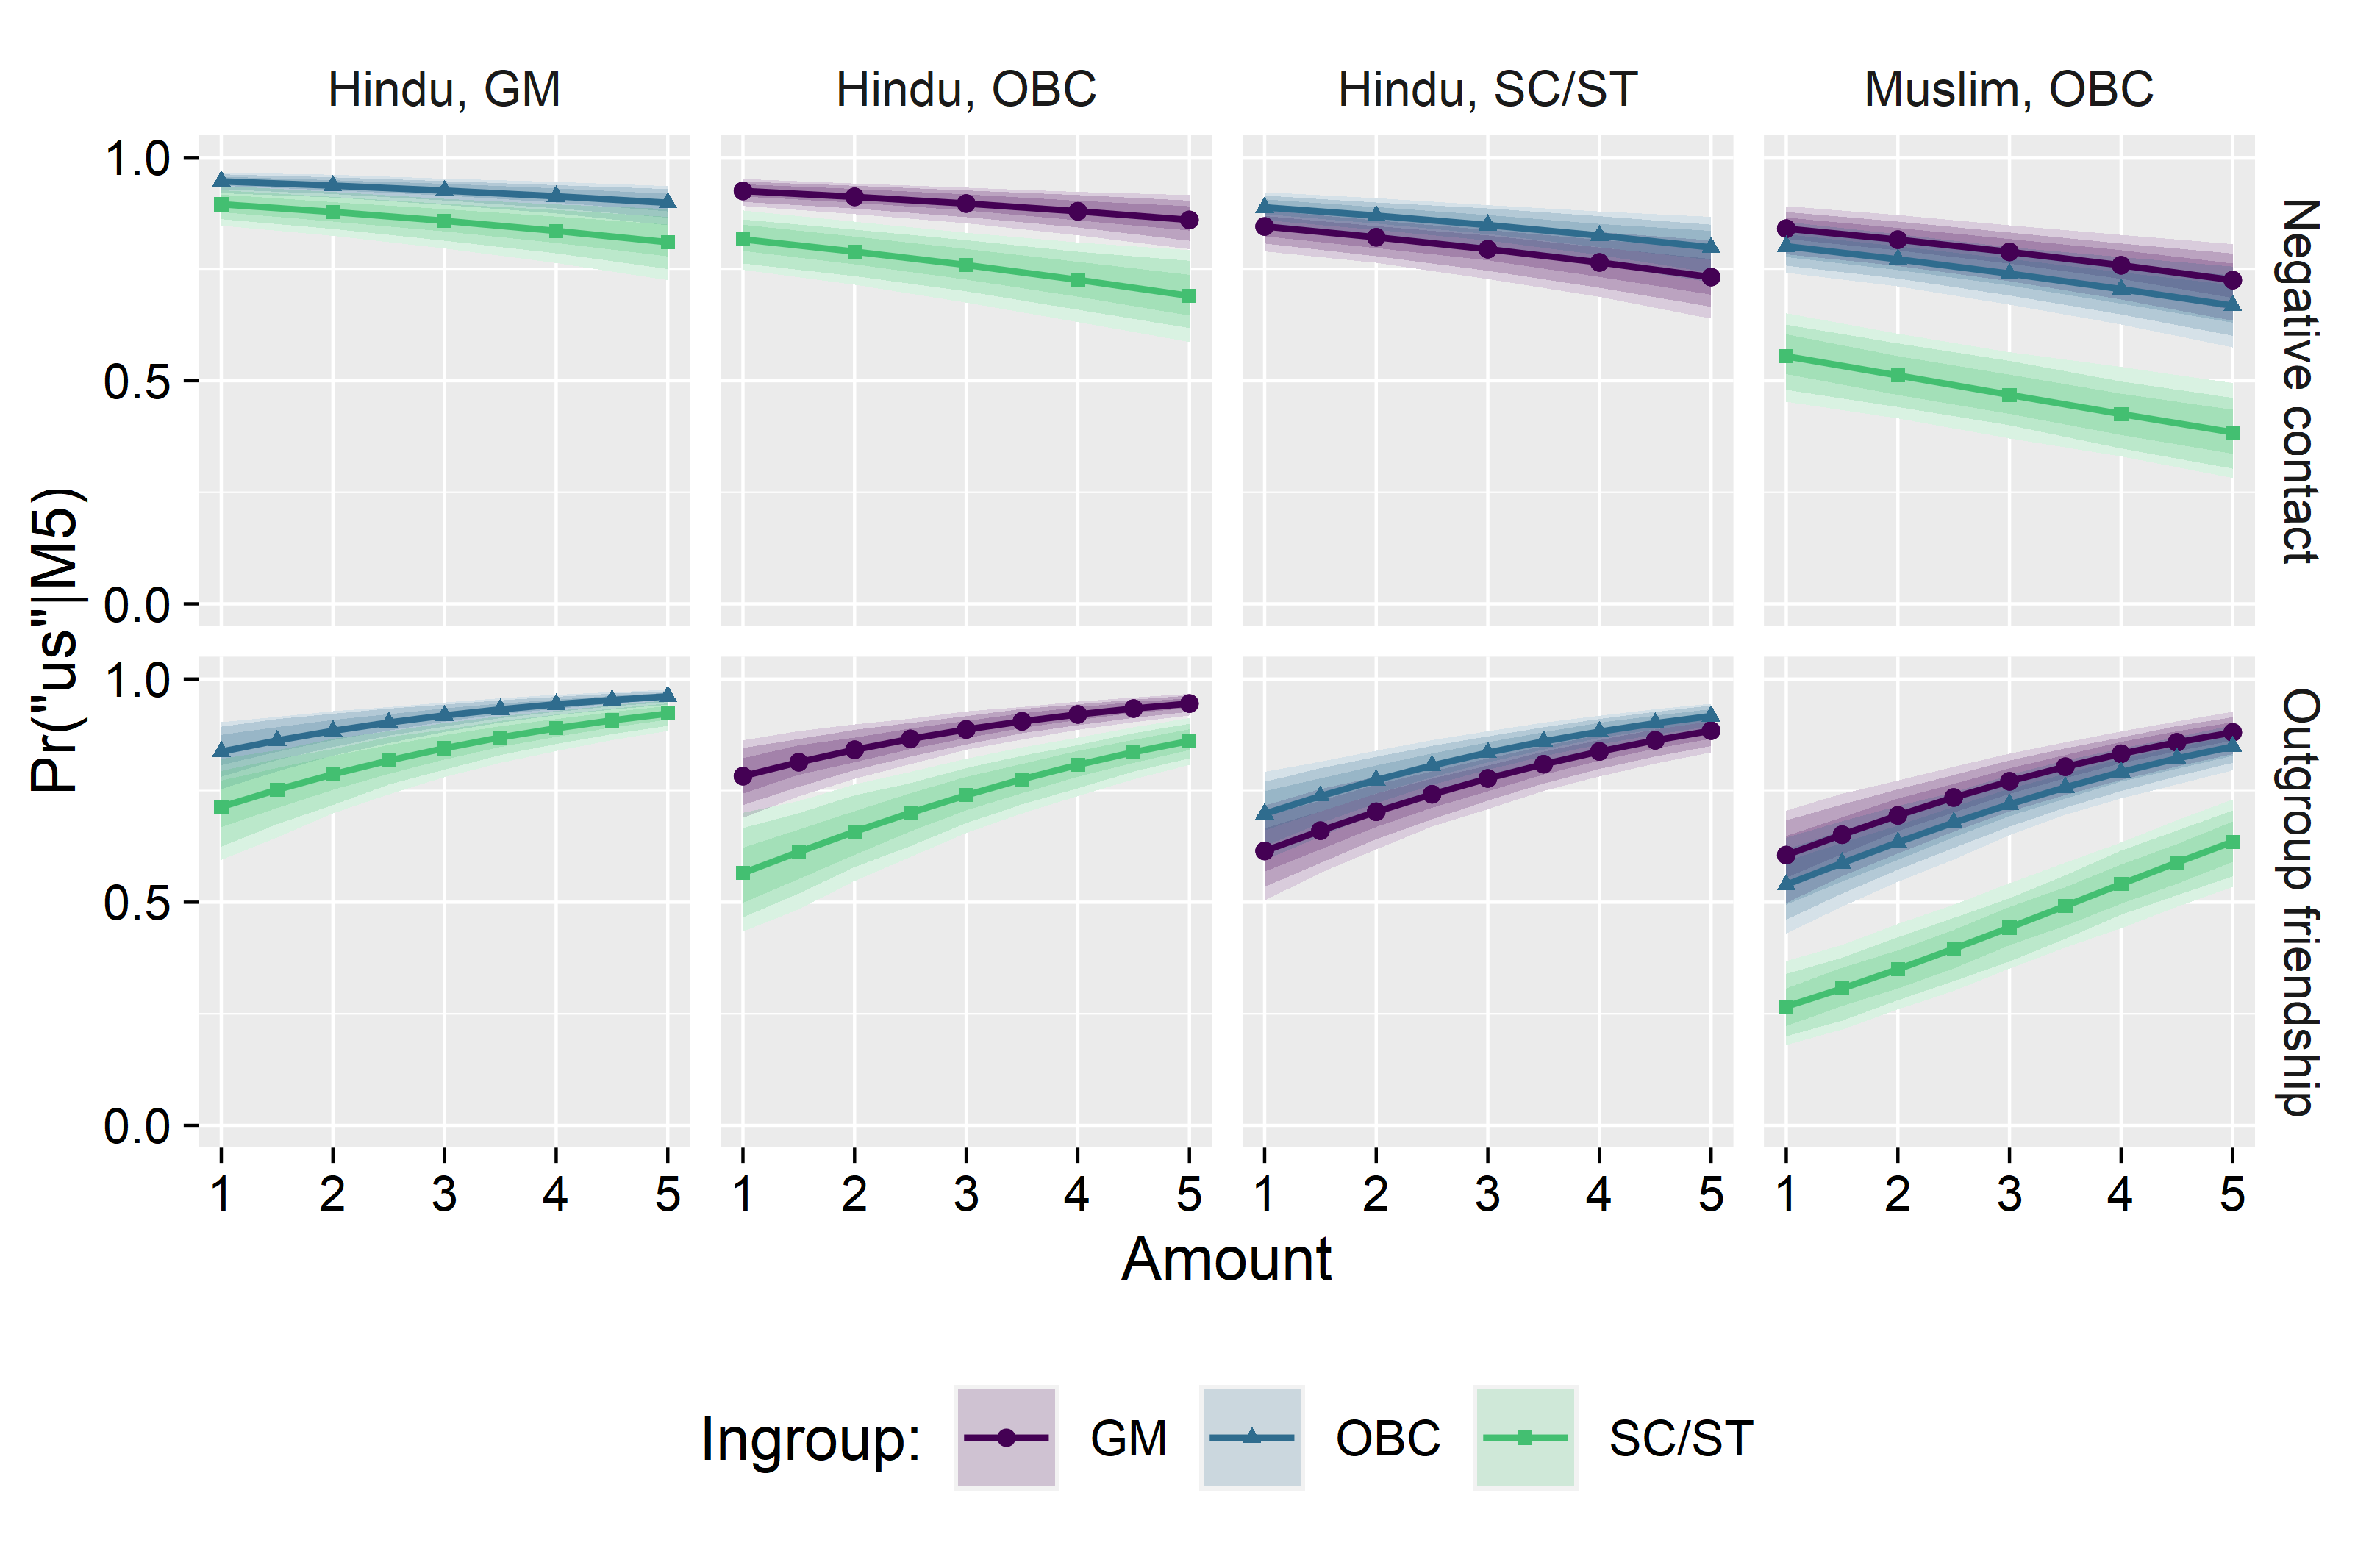
\includegraphics[scale=1]{../figures/figure-4}
\caption{Estimated probability of participants categorising a target as ``us'' versus ``not us'' as a function of the targets' group memberships (horizontal), the participants' group memberships (colour), and the reported amount of negative contact and outgroup friendship with the relevant groups (in Model~5, Table~\ref{tab:t2}). GM = General Merit, OBC = Other Backward Class, SC/ST = Scheduled Caste/Scheduled Tribe.}
\label{fig:f4}
\end{figure}

\begin{table}
\caption{Comparison of models estimating participants' social distance (SD) and feeling thermometer (FT) ratings for each target as a function of group differences and target categorizations. As in Table~\ref{tab:t2}, we selected a more complex model over a simpler model when $\frac{\Delta\textit{ELPD}}{\textit{SE}} \geq 2$. $R^2$ is a Bayesian analogue to $R^2$ in maximum likelihood estimation (Gelman, Goodrich, Gabry, \& Ali, 2017).}
\centering
\figureversion{lining, tabular}
\small	
\begin{tabularx}{\linewidth}{r@{~}rXrrrrrrrr} \toprule
\# &  & Description & $R^2_\text{SD}$ & $R^2_\text{FT}$ & $\textit{ELPD}$ & $\textit{SE}$ & $\Delta\textit{ELPD}$ & $\textit{SE}$ & $\frac{\Delta\textit{ELPD}}{\textit{SE}}$ & $w$ \\ \midrule 
0 &      & Participant & .23 & .26 & -16964 & 71.0 & - & - & - & .12 \\
1 & vs 0 & Category & .38 & .42 & -16338 & 79.6 & 626.8 & 40.2 & 15.6 & .02 \\
2 & vs 1 & SC/ST    & .38 & .43 & -16317 & 79.6 &  20.1 &  9.8 &  2.1 & .00 \\
3 & vs 2 & OBC      & .39 & .43 & -16293 & 80.5 &  24.2 &  9.7 &  2.5 & .00 \\ \midrule
4 & vs 3 & Categorization    & .42 & .47 & -16028 & 83.5 & 264.8 & 24.5 & 10.8 & .19 \\
5 & vs 4 & \ldots~(Category) & .42 & .47 & -16007 & 83.6 &  21.1 &  8.7 &  2.4 & .67 \\
6 & vs 5 & \ldots~(Ingroup)  & .42 & .47 & -16025 & 84.3 & -17.4 &  5.9 & -3.0 & .00 \\
\bottomrule    
\end{tabularx}
\label{tab:t3}
\end{table}

\begin{figure}
\centering
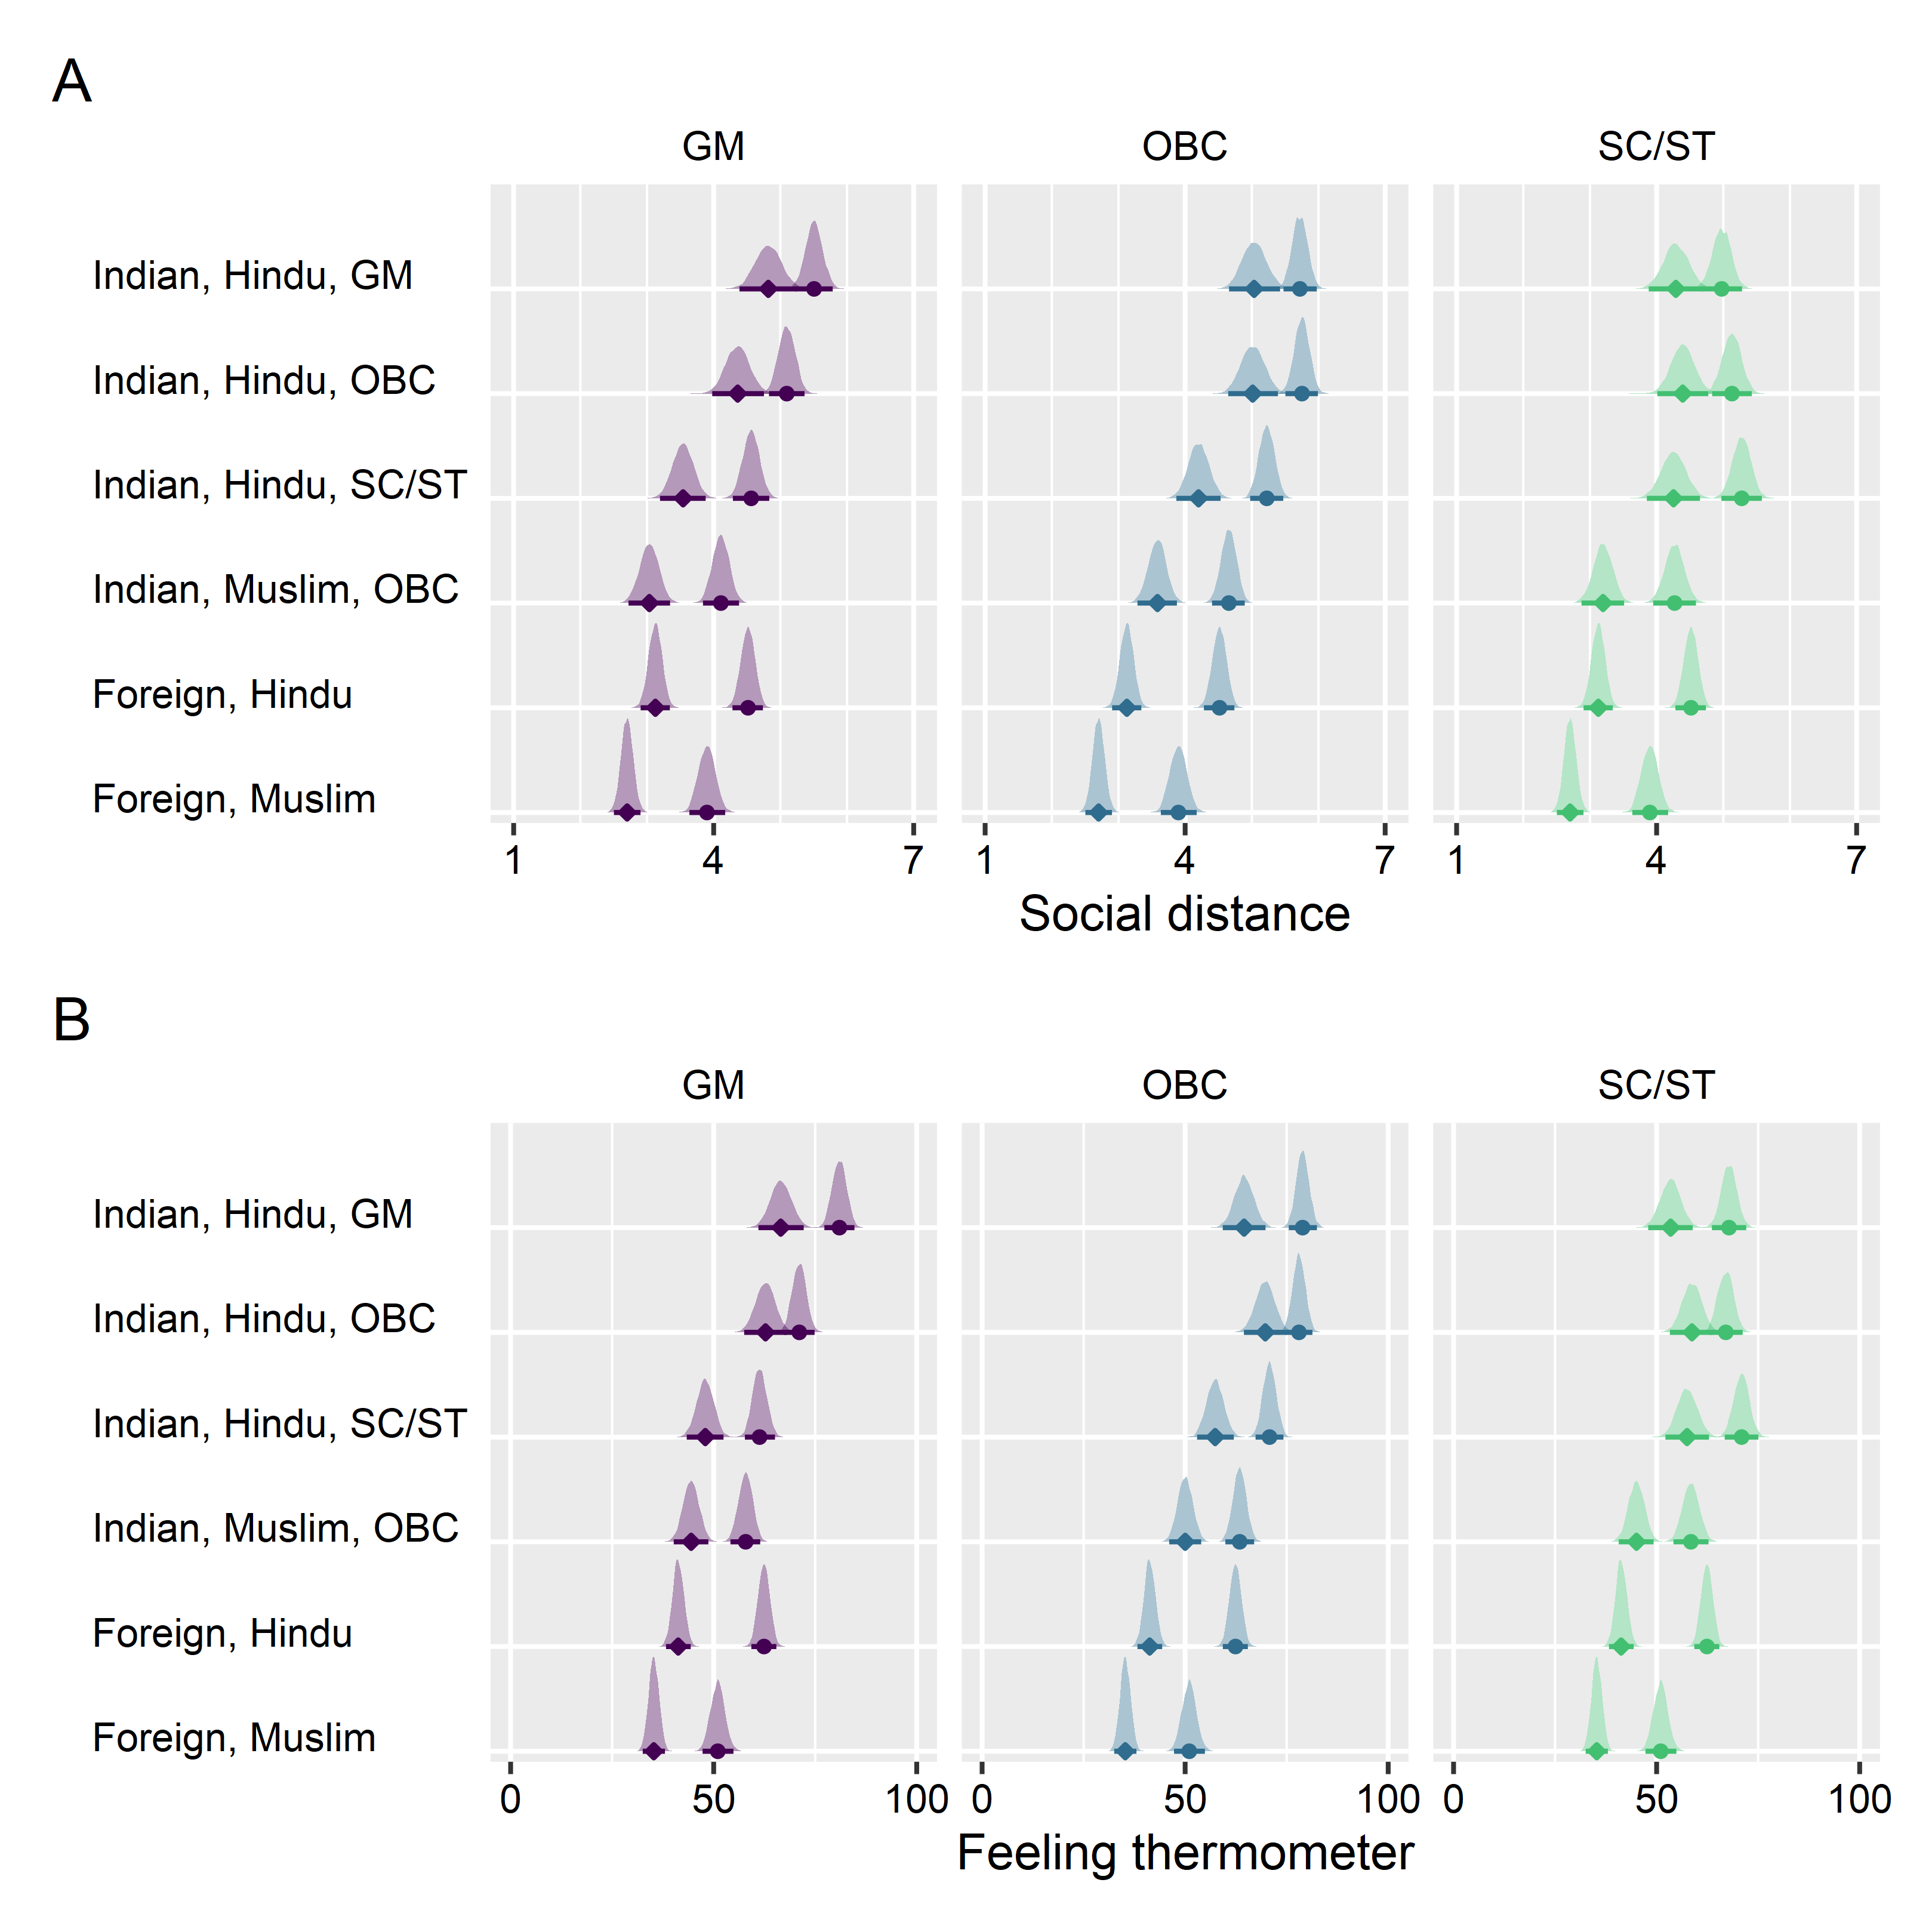
\includegraphics[scale=1]{../figures/figure-5}
\caption{
Posterior probabilities of social distance ratings as a function of target categorizations (in Model 5, Table~\ref{tab:t3}). Points are the estimated mean ratings for targets categorized as ``us''; triangles are the estimated mean ratings for targets categorized as ``not us''. GM = General Merit, OBC = Other Backward Class, SC/ST = Scheduled Caste/Scheduled Tribe.
}
\label{fig:f5}
\end{figure}

\begin{figure}
\centering
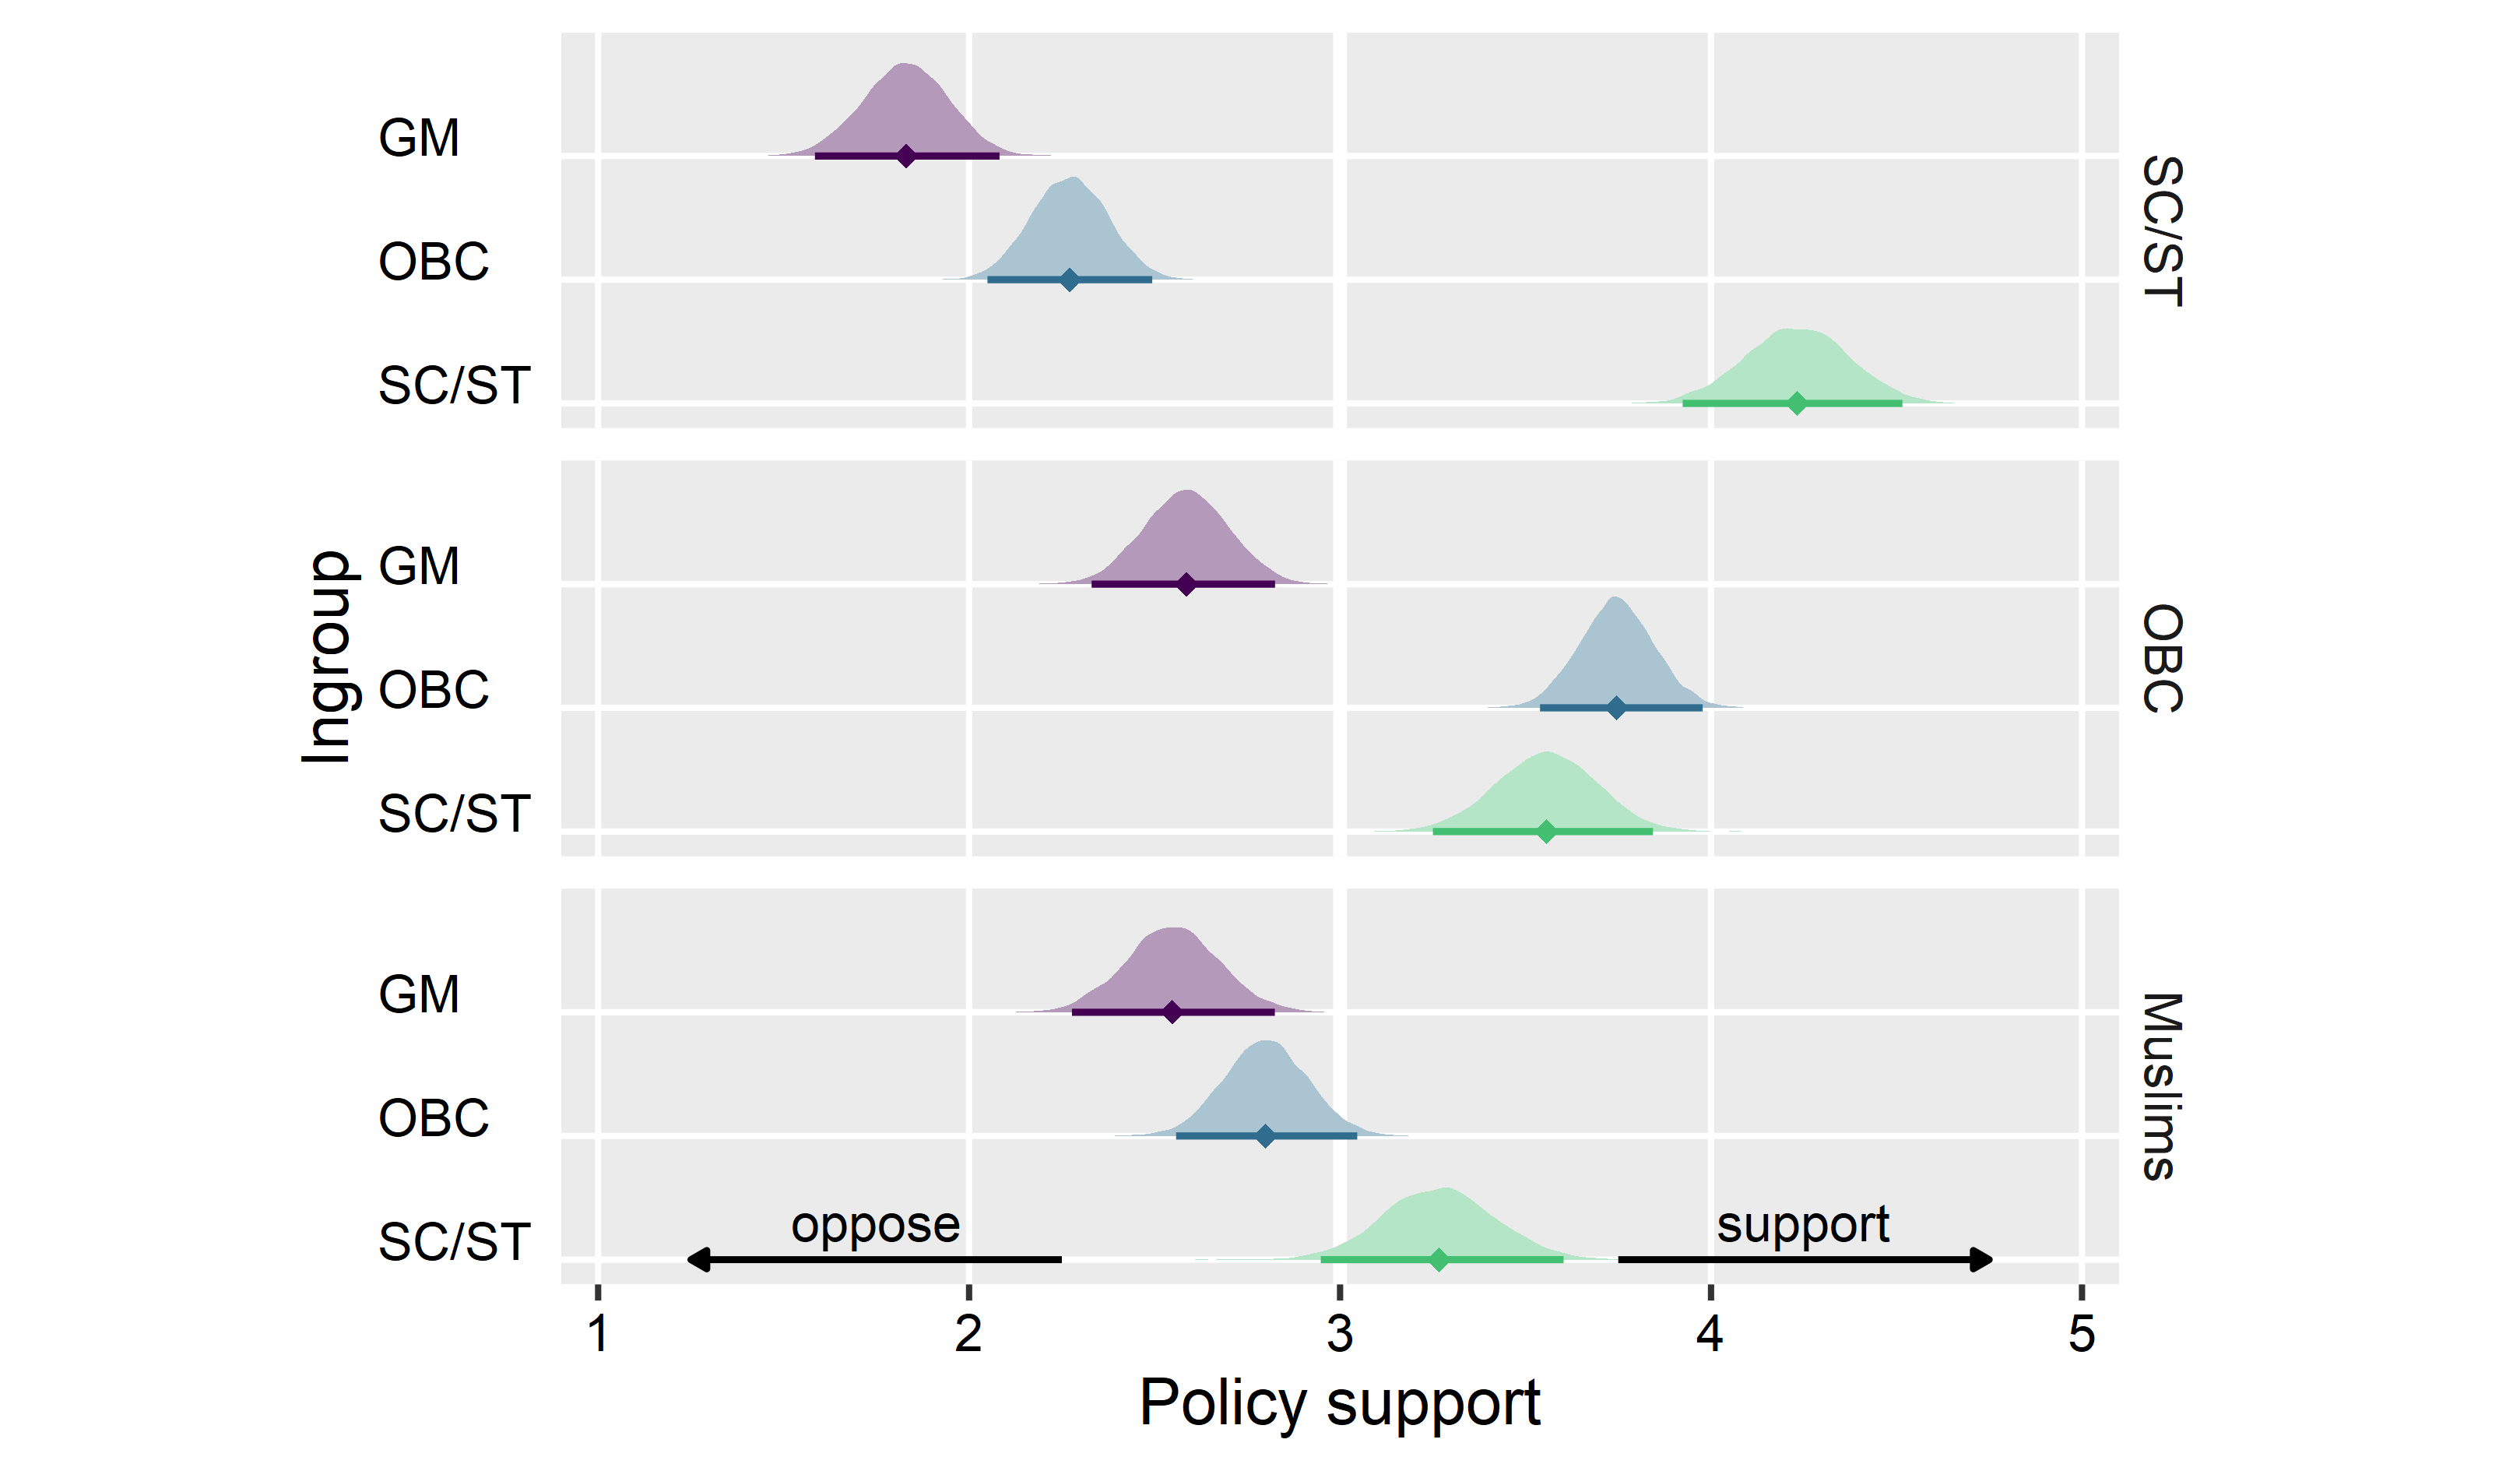
\includegraphics[scale=1]{../figures/figure-6}
\caption{
Posterior probabilities of feeling thermometer ratings as a function of target categorizations (in Model 5, Table~\ref{tab:t3}). Points are the estimated mean ratings for targets categorized as ``us''; triangles are the estimated mean ratings for targets categorized as ``not us''. GM = General Merit, OBC = Other Backward Class, SC/ST = Scheduled Caste/Scheduled Tribe.
}
\label{fig:f6}
\end{figure}

\begin{figure}
\centering
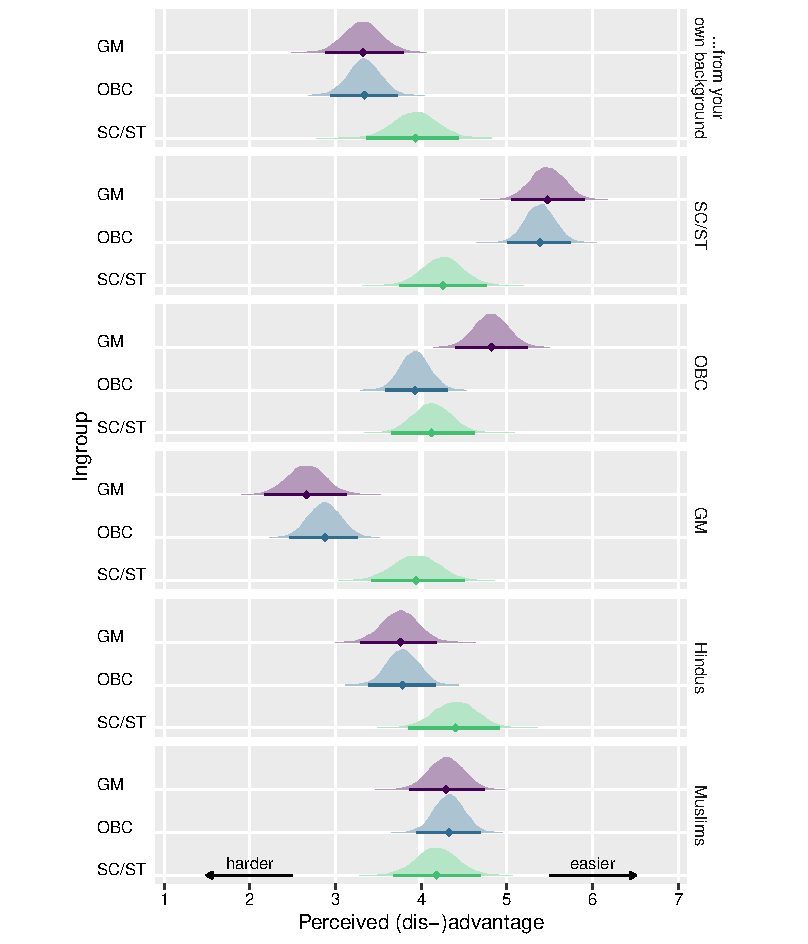
\includegraphics[scale=1]{../figures/figure-7}
\caption{
Posterior probabilities of perceived life difficulty ratings for different target groups (right) by participants' caste ingroup (left). Diamonds mark the most plausible estimate of each mean rating; intervals encompass the 97\% most plausible estimates. GM = General Merit, OBC = Other Backward Class, SC/ST = Scheduled Caste/Scheduled Tribe.
}
\label{fig:f7}
\end{figure}

\begin{figure}
\centering
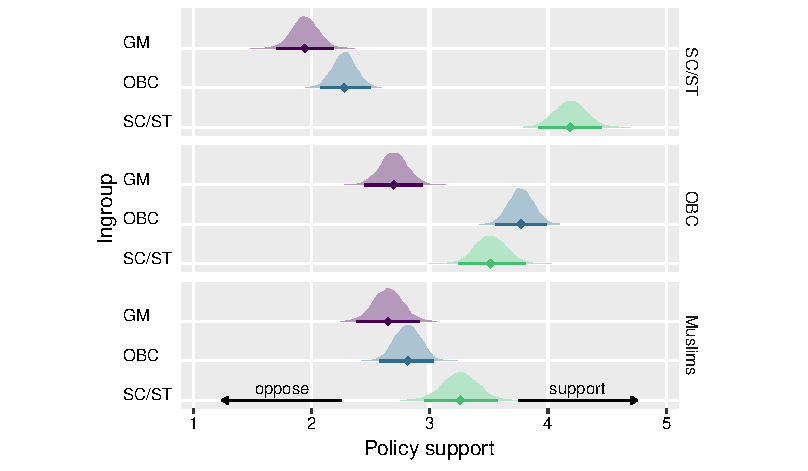
\includegraphics[scale=1]{../figures/figure-8}
\caption{
Posterior probabilities of policy support ratings for different target groups (right) by participants' caste ingroup (left). Diamonds mark the most plausible estimate of each mean rating; intervals encompass the 97\% most plausible estimates. GM = General Merit, OBC = Other Backward Class, SC/ST = Scheduled Caste/Scheduled Tribe.
}
\label{fig:f8}
\end{figure}

\end{document}